\documentclass[9pt]{ltjsreport}
\usepackage{bm}
\usepackage{amsmath,amssymb}
\usepackage{tcolorbox}
\usepackage{graphicx}
\usepackage{booktabs}
\usepackage{subcaption}
\usepackage{tikz}
\usepackage{listings}
\usetikzlibrary{graphs}

\begin{document}

\chapter{数理計画}
\section{数理計画モデル}
\subsection{数理計画とは}
制約条件の元、目的関数を最大化するような問題
\subsection{線形計画問題とは}
数理計画問題のうち、目的関数が線形かつ、制約条件が線形の等式または
不等式であるもの。


\subsection{以下の線形計画問題のモデル化を行え}
\subsubsection{以下の生産計画問題に対し、そのモデル化を行え}
    4種類の原料A,B,C,Dをもちいて、三種の製品x,y,zを生産する工場を考える。
    そして図\ref{tab:productiveplan}のように製品を生産するために必要な原材料の量が定義されている
    とする。

    そして、現時点で、Aを80、Bを50、Cを100、Dを70単位持っているとする。

    また、xは70、yは120、zは30万円で売れるとする。

\begin{table}[h]
    \centering
    \caption[生産計画問題のデータ]{各製品を１単位生産するために必要な各原料の量}
    \label{tab:productiveplan}
    \begin{tabular}{cccc}\toprule
         &x&y&z\\ \midrule
        A&5&0&6\\
        B&0&2&8\\
        C&7&0&15\\
        D&3&11&0\\\bottomrule
    \end{tabular}
\end{table}
    このような場合に、最大の利益を上げる生産計画はどのように立てればよいか。

    \hrulefill

製品x,y,zの生産量をそのままx,y,zとする。

このとき、上の生産計画問題は、
目的関数$70x+120y+30z$を以下の制約条件のもと最大化することと同じである。

\begin{equation}
\begin{matrix}
        5x&   &+6z &\ge&80\\
          & 2y&+8z &\ge&50\\
        7x&   &+15z&\ge&100\\
        3x&+11y&   &\ge&70
\end{matrix}
\hspace{1cm} (\text{原料による制約})
\end{equation}
\begin{equation}
    x\ge 0,y\ge 0,z\ge 0 \hspace{1cm} (\text{非負条件} )
\end{equation}

\newpage
\subsubsection{以下の多期間計画問題に対し、そのモデル化を行え}
工場は2種類の原料A,Bを加工して2種類の製品x,yを生産しているとする。

そして、以下のようなデータが与えられているとする。
\begin{table}[h]
    \centering
    \label{tab:manySpan}
    \caption{多期間計画問題のデータ}
    \begin{subfigure}{0.2\columnwidth}
        \centering
        \caption[(a)]{単位製品あたりの原料使用量}
        \begin{tabular}{ccc}\toprule
             &x&y\\ \midrule
            A&2&7\\
            B&5&3 \\ \bottomrule
        \end{tabular}
    \end{subfigure}
    \begin{subfigure}{0.2\columnwidth}
        \centering
        \caption[(b)]{製品の出荷量}
        \begin{tabular}{ccc}\toprule
             &x&y\\ \midrule
            1月&30&20\\
            ２月&60&50 \\
            3月&80&90\\ \bottomrule
        \end{tabular}
    \end{subfigure}
    \begin{subfigure}{0.2\columnwidth}
        \centering
        \caption[(c)]{原料の利用可能料}
        \begin{tabular}{ccc}\toprule
             &A&B\\ \midrule
            1月&920&790\\
            2月&750&600 \\
            3月&500&480 \\ \bottomrule
        \end{tabular}
    \end{subfigure}
    \begin{subfigure}{0.2\columnwidth}
        \centering
        \caption[(d)]{生産コストと在庫コスト}
        \begin{tabular}{ccc}\toprule
             &x&y\\ \midrule
            生産コスト&75&80\\
            在庫コスト&8&7 \\ \bottomrule
        \end{tabular}
    \end{subfigure}

\end{table}

このとき、(b)の出荷ノルマを満たしながら
コストが最小になるように、各月の生産計画を建てるにはどうすればいいか。

\hrulefill

t月における製品iの生産量を$p_{it}$とおく。(t=1,2,3 :i=x,y)

次に、t月から翌月に持ち越す製品iの在庫量を$s_{it}$とおく。

次に、目的関数を(d)から導き、制約条件として非負条件、原材料の利用可能料に
関する制約条件、出荷ノルマの制約条件を作ればいい。

目的関数が、
\begin{equation*}
    75(\sum_{i=1}^3 p_{xi})
    +80(\sum_{i=1}^3 p_{yi})
    +8(\sum_{i=1}^2 s_{xi})
    +7(\sum_{i=1}^2 s_{yi})
    \longrightarrow \min
\end{equation*}
として、利用可能条件が、
\begin{gather*}
    2p_{x1}+7p_{y1}\le 920\\
    5p_{x1}+3p_{y1}\le 790\\
    2p_{x2}+7p_{y2}\le 750\\
    5p_{x2}+3p_{y2}\le 600\\
    2p_{x3}+7p_{y3}\le 500\\
    5p_{x3}+3p_{y3}\le 480
\end{gather*}
となり、出荷量から導かれる制約条件は次のように書ける。
\begin{gather*}
    p_{x1}-s_{x1}=30\\
    p_{y1}-s_{y1}=20\\
    s_{x1}+p_{x2}-s_{x2}=60\\
    s_{y1}+p{y2}-s_{y2}=50\\
    s_{x2}+p_{x3}=80\\
    s_{y2}+p_{y3}=90
\end{gather*}
更に、p,sに対して非負条件が以下のように課せられる。
\begin{equation*}
    p_{ij},s_{ik}\ge 0 \text{(i=x,y  j=1,2,3 k=1,2)}
\end{equation*}
\newpage
\subsubsection{以下の輸送問題に対し、そのモデル化を行え}
この問題は線形計画門でもあるが、
グラフで表現できるネットワーク問題でもあることに留意する。

２つの工場$A_1,A_2$で生産された商品が、３つの取引先$B_1,B_2,B_3$
に納入されている状況を考える。

工場の生産量、取引先の注文量、工場から取引先への輸送コストを下の図に示す。

\begin{table}[h]
    \centering
    \label{tab:transportation}
    \caption{輸送問題のデータ}
    \begin{subfigure}{0.3\columnwidth}
        \centering
        \caption[(a)]{注文料}
        \begin{tabular}{c|c}\toprule
            B1&70\\
            B2&40\\
            B3&60 \\ \bottomrule
        \end{tabular}
    \end{subfigure}
    \begin{subfigure}{0.3\columnwidth}
        \centering
        \caption[(b)]{生産量}
        \begin{tabular}{c|c}\toprule
            A1&90\\
            A2&80\\ \bottomrule
        \end{tabular}
    \end{subfigure}
    \begin{subfigure}{0.3\columnwidth}
        \centering
        \caption[(c)]{輸送コスト}
        \begin{tabular}{cccc}\toprule
            &B1&B2&B3\\ \midrule
            A1&4&7&12\\
            A2&11&6&3 \\ \bottomrule
        \end{tabular}
    \end{subfigure}
\end{table}



この時、輸送コストを最小にするためには、どのように輸送計画を立てればよいか。

\hrulefill

工場$A_i$から工場$B_j$への輸送量を$x_{ij}$とする。(i=1,2 j=1,2,3)

目的関数は、輸送コストの総和である、
\begin{equation}
    4x_{11}+7x_{12}+12x_{13}+11x_{21}+6x_{22}+3x_{23}
\end{equation}
となり、以下に示す制約条件の元これを最小化する。

以下のようにいくつかの制約条件が決まる。

生産量に関する条件は、
\begin{gather}
    \sum_{j=1}^3 x_{1j} = 90\\
    \sum_{j=2}^3 x_{2j} = 80
\end{gather}    

注文量に関する条件は、
\begin{gather}
    x_{11}+x_{21}=70\\
    x_{12}+x_{22}=40\\
    x_{13}+x_{23}=60
\end{gather}

輸送量に関する非負条件として、
\begin{equation}
    x_{ij}\ge 0 (i=1,2 j=1,2,3)
\end{equation}

が考えられる。
\newpage
\subsection{ネットワーク計画問題とは}
グラフ上でフローや枝や節点に
なんらかの属性や数値が与えられている対象を
ネットワークとする。

このようなネットワークで表現できるような
数理計画問題を問題をネットワーク問題という。

ネットワーク問題の対象となるネットワークとして、以下のようなものを
暗黙に仮定する。
\begin{figure}[h]
\caption{ネットワークの例}
\begin{center}
    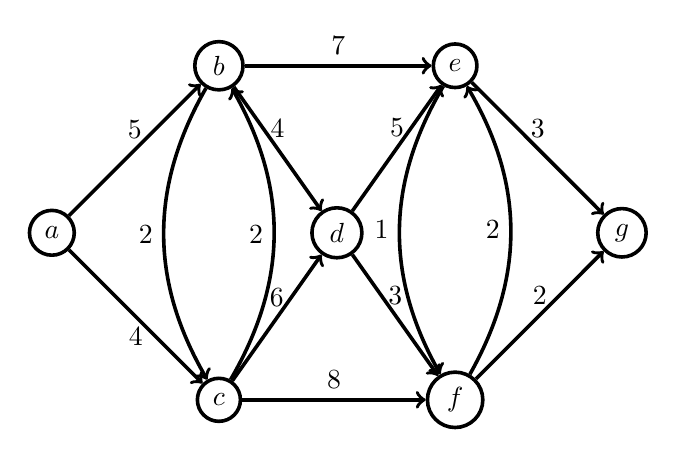
\begin{tikzpicture}[line width=1.3pt,node distance=3cm]
        \node                    (a)[draw,circle]{$a$};
        \node[above right of= a ](b)[draw,circle]{$b$};
        \node[below right of= a ](c)[draw,circle]{$c$};
        \node[right of= a,node distance=3.62cm ](d)[draw,circle]{$d$};
        \node[      right of= b ](e)[draw,circle]{$e$};
        \node[      right of= c ](f)[draw,circle]{$f$};
        \node[right of= a,node distance=7.24cm ](g)[draw,circle]{$g$};
    
        \draw[->](a) -- (b)node[midway,above]{$5$};
        \draw[->](a) -- (c)node[midway,below]{$4$};
    
    
        \draw[->](b) -- (d)node[midway,above]{$4$};
        \draw[->](b) -- (e)node[midway,above]{$7$};
    
     
        \draw[->](c) -- (d)node[midway,above]{$6$};
        \draw[->](c) -- (f)node[midway,above]{$8$};
    
        \draw[->](d) -- (e)node[midway,above]{$5$};
        \draw[->](d) -- (f)node[midway,above]{$3$};
    
    
        \draw[->](e) -- (g)node[midway,above]{$3$};
    
    
        \draw[->](f) -- (g)node[midway,above]{$2$};
    
        \draw[->](b) to[bend right] node[midway,left]{$2$}(c);    
        \draw[->](c) to[bend right] node[midway,left]{$2$}(b);
        \draw[->](f) to[bend right] node[midway,left]{$2$}(e);   
        \draw[->](e) to[bend right] node[midway,left]{$1$}(f);
    
\end{tikzpicture}
\end{center}
\end{figure}

\subsubsection{最短路問題とその定式化をせよ}
ネットワークを交通機関の路線とみなし、
枝の横に書かれている数値をその路線を利用したときの所要時間とみなす。

このとき、あるノードから別のノードへの路のうち、
最小の所要時間を持つ路を選ぶのが最小路問題である。
最小経路問題を下で定義された0-1条件を使って定式化せよ。
\begin{tcolorbox}[title=0-1条件]
    \begin{equation}
        x_{ij}=\begin{cases}
            1 , \text{(i,j)を通る}\\
            0 , \text{(i,j)を通らない}
        \end{cases}
    \end{equation}
\end{tcolorbox}

\hrulefill

路(i,j)が持つ数値を$a_{ij}$とおく。すると、
目的関数は、
\begin{equation}
    \sum_{(i,j)} a_{ij}x_{ij}
\end{equation}

と書ける。
制約条件は、0-1条件で、枝が出ていく数
と枝が入る数がちょうどよくなるように設定する。
すなわち、
\begin{equation*}
    \begin{cases}
    \sum_ix_{in}=1\text{ (ノードnが始点の時)}\\
    \sum_ix_{in}-\sum_ix_{ni}=0\text{(ノードnが始点でも終点でもない時)}\\
    \sum_ix_{ni}=1\text{(ノードnが終点の時)}
    \end{cases}
\end{equation*}


\newpage

\subsection{非線形計画モデルとは}
目的関数や制約条件の中に非線形の関係が出てくるもの
\subsubsection{以下に示す資源配分問題の定式化を示せ}
資源配分関数は、資源の割当を考える問題である。

資源配分問題の一例として、試験勉強のシチュエーションを考える。

試験まで時間がTあるとする。
試験科目は3つあり、それぞれに時間を注ぎ込めば
図\ref{fig:ResourceFunc}のように非線形の形で得点が上昇するものとする。
3つの科目について、勉強時間と得点の関係を
$h_1(t),h_2(t),h_3(t)$として表すことができると仮定する。

このような場合に、３科目の得点の合計が最大になるように勉強時間を配分するにはどうすればよいか。

\begin{figure}[h]
    \caption{資源配分関数(非線形)}
    \label{fig:ResourceFunc}
\begin{center}
\begin{tikzpicture}[domain=0:1.5,samples=200,x=3cm,y=3cm]
    \draw[->] (0,0) -- (1.5,0) node[right]{資源t};
    \draw[->] (0,0) -- (0,1) node[above]{成果h};
    \draw plot (\x,{sqrt(\x)}) node[below]{$h=\sqrt{t}$};
\end{tikzpicture}
\end{center}
\end{figure}

\hrulefill

上の資源配分問題は下のように定式化できる。

科目$h_1,h_2,h_3$にかかる時間を$t_1,t_2,t_3$と置く。
\begin{gather*}
    \text{目的関数：}h_1(t_1)+h_2(t_2)+h_3(t_3)\longrightarrow \max\\
    \text{制約条件：}t_1+t_2+t_3=T, t_i\ge0(i=1,2,3)
\end{gather*}

\subsubsection{ポートリフォ選択問題とは何かとその定式化を示せ}
ポートリフォ選択問題とは、投資家が資産を投資判断を
するためにはどうするべきかを考える問題である。

投資家は現在w円をもち、３種の株式$A_1,A_2,A_3$に分散して投資しようとしている。
株式$A_1,A_2,A_3$の（一株あたりの）現在価格は$p_1,p_2,p_3$と仮定する。

このような状況下で、利益を出すにはどうすれば良いか。


\hrulefill

各株式への投資額を$x_1,x_2,x_3$と置く。

すると、制約条件が
\begin{gather}
    x_1+x_2+x_3=w\\
    x_1,x_2,x_3\ge 0
\end{gather}
となる。

一ヶ月後の株式$A_1,A_2,A_3$の価格を確率変数$P_1,P_2,P_3$で表すとする。

このとき、一ヶ月後の資産の総額は、
\begin{equation}
    W:=\sum_{i=1}^3 \frac{P_ix_i}{p_i}
\end{equation}
の確率変数で表現ができる。

得られる利益は、$W-w$なので、

\begin{align}
    Z : & = W-w \notag \\
      & = \sum_{i=1}^3 \frac{P_ix_i}{p_i} - w \notag \\
      & = \sum_{i=1}^3 \frac{P_i - p_i}{p_i} x_i
\end{align}
とかける。

\begin{tcolorbox}[title=収益率の定義]
単位投資額あたりの儲けを表す確率変数を、収益率と定義する。
\begin{equation}
    R_i := \frac{P_i-p_i}{p_i} (i=1,2,3)
\end{equation}
\end{tcolorbox}

このことから、
\begin{equation}
    Z=\sum_{i=1}^3 R_ix_i
\end{equation}
と簡潔に表現可能である。


投資家は利益Zが最大となるように投資を行えば良い。
しかし、Zは確率変数である。

このような不確実性の元で意思決定を行うには、期待効用理論
に基づく最適化規範を導入する。

ここで、実際に得られた利益zで投資家の満足度を表す、
単調増加関数である効用関数u(z)を定義する。

\begin{figure}[h]
    \caption{効用関数(非線形)}
    \label{fig:satisfaction}
\begin{center}
\begin{tikzpicture}[domain=0:1.5,samples=200,x=3cm,y=3cm]
    \draw[->] (0,0) -- (1.5,0) node[right]{利益z};
    \draw[->] (0,0) -- (0,1) node[above]{効用u};
    \draw plot (\x,{sqrt(\x)});
\end{tikzpicture}
\end{center}
\end{figure}

ポートリフォ問題は、ポートリフォ関数の期待値を最大化する問題
として定式化ができる。

\newpage
\subsubsection{交通流割当問題とその定式化を示せ}

図(\ref{fig:transportationflaw})のような
フローとフローを流したときのコスト関数をもつネットワーク。
wのフローをAをソース、Dをシンクとして流すとする。

この時、コストが最小になるようにフローを流すにはどうすればよいか。
\begin{figure}[h]
\centering
\caption{フローを持つネットワーク}
\label{fig:transportationflaw}
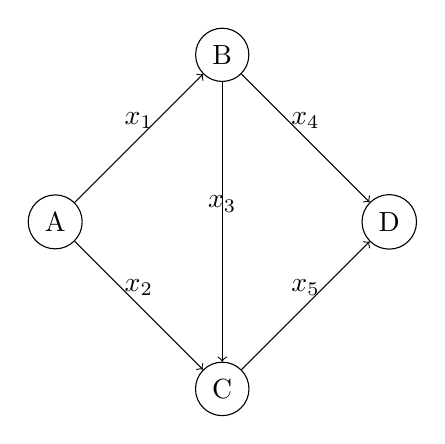
\begin{tikzpicture}[node distance = 3cm]
    \node(a)        [draw,circle]{A};
    \node[above right of = a](b)        [draw,circle]{B};
    \node[below right of = a](c)        [draw,circle]{C};
    \node[above right of = c](d)        [draw,circle]{D};

    \draw[->](a) -- node[midway,above]{$x_1$}(b);
    \draw[->](a) -- node[midway,above]{$x_2$}(c);
    \draw[->](b) -- node[midway,above]{$x_3$}(c);
    \draw[->](b) -- node[midway,above]{$x_4$}(d);
    \draw[->](c) -- node[midway,above]{$x_5$}(d);
\end{tikzpicture}
\end{figure}

\hrulefill

図\ref{fig:transportationflaw}のように枝に与える数値として
変数$x_1,\dots,x_5$を定義する。
また、この数値は道路を利用する車の台数を意味するとする。

このことから、制約条件が以下のように定まる。

Aから出てくる数、Dに入る数はwなので
\begin{gather}
    x_1+x_2=w\\
    x_4+x_5=w
\end{gather}
出てくる数と入る数は等しいので、
\begin{gather}
    x_1=x_3+x_4\\
    x_2+x_3=x_5
\end{gather}
また、非負条件から、
\begin{equation}
    x_i \ge 0 (i=1,\dots,5)
\end{equation}

数値$x_i$をもつ路のコスト関数を、$f_i(x_i)$
と置く。

このとき、フローによるコストは
\begin{equation}
    \sum_{i=1}^5=x_if_i(x_i) \label{eq:sumTransportation}
\end{equation}
となる。
まとめると、\ref{eq:sumTransportation}を上の制約条件
のもとで最小化するような$x_1,\dots,x_5$をみつければよい。

\subsubsection{システム最適とユーザ最適とは}
\begin{tcolorbox}[title=システム最適]
    交通流割当問題のように、システムに対して行う
    最適化
\end{tcolorbox}
\begin{tcolorbox}[title=ユーザ最適]
    ユーザ毎に最適化すること
\end{tcolorbox}

\subsection{整数計画問題とは}
線形計画問題のうち、変数の各要素が整数に限定されるもの

整数計画問題は、変数が整数値に限定されたことにより、問題
が格段に難しくなる。

\subsubsection{固定費付き輸送問題の定式化をせよ}
この問題は輸送問題に酷似している。

２つの倉庫$A_1,A_2$から$B_1,B_2,B_3$へ注文を満たす
ように品物を送る場合を考える。
その際、以下のようなデータが与えられているものとする。
\begin{table}[h]
    \centering
    \caption{固定費付き輸送問題のデータ}
    \begin{subfigure}{0.3\columnwidth}
        \centering
        \caption{注文量}
        \begin{tabular}{cc}\toprule
              &注文量\\ \midrule
            B1&20\\
            B2&30\\
            B3&15\\ \bottomrule
        \end{tabular}
    \end{subfigure}
    \begin{subfigure}{0.3\columnwidth}
        \centering
        \caption{輸送コスト}
        \begin{tabular}{cccc}\toprule
              &B1&B2&B3\\ \midrule
            A1&5&3&2\\
            A2&2&7&4\\ \bottomrule
        \end{tabular}
    \end{subfigure}
    \begin{subfigure}{0.3\columnwidth}
        \centering
        \caption{固定費}
        \begin{tabular}{cc}\toprule
              &固定費\\ \midrule
            A1&300\\
            A2&200\\ \bottomrule
        \end{tabular}
    \end{subfigure}
\end{table}

固定費とは、実際に倉庫を使用するときに、
輸送量の大きさに関係なくかかる額とする。

この際、どのように輸送計画を立てれば輸送コストが
最小になるだろうか。

\hrulefill

倉庫$A_i$から$B_J$への輸送量の変数を$x_{ij}$とする。
このとき、各倉庫に対する費用は0-1変数

\begin{align}
    y_i=
    \begin{cases}
        1 & \text{倉庫$A_i$を使用するとき}\\
        0& \text{倉庫$A_i$を使用しないとき}
    \end{cases}
\end{align}
を導入すると、

\begin{equation}
    \begin{cases}
        z_1=300y_1+5x_{11}+3x_{12}+2x_{13}\\
        z_2=300y_2+5x_{21}+3x_{22}+2x_{23}\\
    \end{cases}
\end{equation}
で定義できる。

目的関数は、$z_1+z_2$となるので、これを最小化すれば良い。

制約条件は、以下のように定まる。

注文料の総和が65であることから、
\begin{gather}
    \sum^3_{j=1} x_{1j}\le 65y_1 \\
    \sum^3_{j=1} x_{2j}\le 65y_2
\end{gather}
である。

ついでに、非負条件が
\begin{equation}
    x_{ij}\ge0 (i=1,2;j=1,2,3)
\end{equation}
として定まる。

取引先の注文料に対する条件で、
\begin{gather}
    x_{11}+x_{21}=20\\
    x_{12}+x_{22}=30\\
    x_{13}+x_{23}=15
\end{gather}
となる。

\subsubsection{ナップサック問題の定式化をせよ}
重さと価値が異なる品物がn個あるとする。

品物iの重さは$w_i$、価値を$v_i$とする。

今持てる総重量がwのとき、価値の合計が最大となるように品物を選ぶにはどうすればいいか。

\hrulefill

各品物i($i=1,\dots,n$)に対して、0-1変数
\begin{equation}
    x_i=
    \begin{cases}
        1 \text{ (品物iを選ぶとき)}\\
        0 \text{ (品物iを選ばないとき)}
    \end{cases}
\end{equation}

すると、問題は制約条件
\begin{equation}
    \sum_{i=1}^n w_ix_i\le w 
\end{equation}
のもと、目的関数
\begin{equation}
    \sum_{i=1}^n v_ix_i
\end{equation}
を最大化する整数計画問題と考えられる。

\subsection{数理計画問題の定式化を行え}
\begin{tcolorbox}[title=数理計画問題]
\begin{gather*}
    \text{目的関数}:f(\bm{x}) \longrightarrow \text{最大あるいは最小}\\
    \text{制約条件}:\bm{x}\in \bm{S}
\end{gather*}
\end{tcolorbox}
今まで話してきた問題は全て、上の形で表現することができる。


\end{document}